\documentclass[11pt]{article}
\usepackage[margin=1in]{geometry}
\usepackage{graphicx}
\usepackage{amsmath,amssymb}
\usepackage{booktabs}
\usepackage[numbers,sort&compress]{natbib}  % MRM: numbered (Vancouver) references
\usepackage{xcolor}
\usepackage[colorlinks=true,linkcolor=blue,citecolor=blue,urlcolor=blue]{hyperref}
\usepackage{microtype}
\usepackage{caption}
\emergencystretch=2em

\newcommand{\Dstar}{D^{*}}
\newcommand{\unit}[1]{\,\mathrm{#1}}
% Multi-seed empirical [5,95] confidence band (16 seeds; see Sec.~\ref{sec:consistency}).
\newcommand{\band}[2]{{\scriptsize\,$[#1,\,#2]$}}

\title{\textbf{Distribution-Free Conformal Coverage for IVIM Parameter
Maps, and the Identifiability Wall in the Pseudo-Diffusion Compartment}}
\author{Avery Karlin\\[2pt]
\small The Annealing Signet Institute\\[3pt]
\small \textit{Avery Karlin is a graduate student at Columbia University,}\\[1pt]
\small \textit{Department of Applied Physics and Mathematics, and the}\\[1pt]
\small \textit{University of Colorado Boulder, Department of Computer Science.}\\[3pt]
\small ORCID: \href{https://orcid.org/0000-0003-3848-6782}{0000-0003-3848-6782}}
\date{}

\begin{document}
\maketitle

\begin{abstract}
\noindent
\textbf{Purpose:} To establish and characterize the identifiability
limit that governs per-voxel uncertainty in the ill-posed pseudo-diffusion
compartment ($\Dstar$) of intravoxel incoherent motion (IVIM) imaging -- using
distribution-free conformal prediction both as the finite-sample coverage tool
that model-based uncertainty quantification (UQ) lacks and as the lens that
exposes where label-free conditioning cannot succeed -- and to benchmark that
conformal layer head-to-head against model-based IVIM UQ.

\noindent
\textbf{Methods:} On a controlled, seeded synthetic cohort built from our own
bi-exponential forward model with Rician noise, we compare split-conformal and
conformalized quantile regression (CQR) against four model-based baselines
(probabilistic neural network, mixture-density deep ensemble, deep ensemble,
per-voxel Bayesian MCMC), measuring marginal and (SNR $\times$
true-$\Dstar$-tercile) conditional coverage and sharpness, with empirical
$[5,95]$ confidence bands on the conditional quantities from a 16-seed re-run. A
Fisher-information / Cram\'er--Rao analysis diagnoses the residual gap; weighted
(nonexchangeable) conformal and a label-free deployment monitor stress
exchangeability; a qualitative in-vivo demonstration is included.

\noindent
\textbf{Results:} Among credible model-based baselines (MDN deep
ensemble, per-voxel Bayesian MCMC), marginal overconfidence is mild and broad
rather than $\Dstar$-specific (gaps $0.024$--$0.045$); a deliberately weak point
ensemble under-covers severely and is reported only to show the conformal layer
restores coverage from a poor base. The naive $\Dstar$-concentrated hypothesis is
rejected, and the conformal layer's value is the finite-sample guarantee, not the
magnitude of correction. Conformal and conformalized methods restore near-nominal
marginal coverage everywhere ($|\text{gap}|\le 0.024$), and conformalizing the MDN
is the sharpest valid recipe ($0.65$--$0.77\times$ pure-CQR width). The real
failure is conditional: the high-$\Dstar$ regime under-covers for every method we
tested (robustly at low-to-moderate SNR). The barrier is latent-axis conditioning
-- coverage conditional on the true $\Dstar$ regime, an axis the data do not reveal
-- i.e.\ the IVIM instance of the known impossibility of distribution-free
conditional coverage~\citep{barber2021limits}. A Fisher-information /
Cram\'er--Rao analysis shows $\Dstar$ point-identifiability also collapses in the
same regime (the CRLB reaches the regime-bin width): a concomitant diagnostic, not
the proven cause of the coverage failure.
The wall is robust to the b-value scheme; weighted conformal recovers covariate
shift but not forward-model misspecification; the monitor fires before coverage
fails but is blind to the latent gap. The wall is not an artifact of our generator:
a deliberately biased shrinkage estimator buys $\Dstar$ point precision in the
identified terciles without lifting high-$\Dstar$ conditional coverage, and the gap
replicates when the ground truth is a genuinely non-bi-exponential
(velocity-dispersion) mechanism; we additionally chart the off-model validity
envelope across three deviation families, with a graceful, partly monitored
degradation and a recovered bi-exponential origin, and confirm the wall persists
under a clinically realistic correlated, skewed prior with measurement-level
nuisance, where it concentrates in a clinically rare high-$\Dstar$ tail.

\noindent
\textbf{Conclusion:} The central finding is an IVIM-specific identifiability
boundary: high-$\Dstar$ regime-conditional coverage is unrecoverable by the
label-free methods we tested -- now including a deliberately biased shrinkage
estimator, and replicating under a non-bi-exponential generator -- the IVIM instance
of the established impossibility of distribution-free conditional
coverage~\citep{barber2021limits}. The
Cram\'er--Rao bound, which exceeds the regime resolution here, is a concomitant
point-identifiability diagnostic rather than the demonstrated cause.
Conformal prediction supplies the finite-sample marginal guarantee model-based
IVIM UQ lacks -- and conformalizing a strong base is the sharpest valid recipe --
but its deeper value here is diagnostic: it draws the line the data themselves
impose. We characterize that limit; we do not claim to solve it.
\end{abstract}

\vspace{0.5em}
\noindent\textbf{Keywords:} intravoxel incoherent motion (IVIM); uncertainty
quantification; conformal prediction; identifiability; pseudo-diffusion;
quantitative MRI.

\section{Introduction}
IVIM imaging~\citep{lebihan1988} separates microcirculatory perfusion from tissue
diffusion by fitting the bi-exponential signal
\begin{equation}
\frac{S(b)}{S_0} = f\,e^{-b\Dstar} + (1-f)\,e^{-bD},
\label{eq:ivim}
\end{equation}
where $b$ is the diffusion weighting (s/mm$^2$), $D$ the tissue diffusion
coefficient, $\Dstar \gg D$ the pseudo-diffusion coefficient, and $f$ the
perfusion fraction. Equation~\eqref{eq:ivim} is notoriously ill-posed: $\Dstar$ is
poorly constrained because the fast-decaying perfusion term contributes only at
low $b$, and small perfusion fractions make it nearly unidentifiable. Clinical use
of IVIM parameter maps therefore demands trustworthy \emph{per-voxel uncertainty},
not just point estimates.

The dominant approach to IVIM UQ is \emph{model-based}: probabilistic neural
networks, deep ensembles, mixture-density networks, and Bayesian fitting place a
distribution over parameters and read intervals from it. These methods make
distributional assumptions and carry \emph{no finite-sample coverage guarantee};
the most comprehensive IVIM-UQ study to date~\citep{casali2026} documents that
such models are well-calibrated for $D$ and $f$ but \emph{overconfident in
$\Dstar$}. \emph{Conformal prediction}~\citep{vovk2005,lei2018,angelopoulos2023}
offers the complementary property: under exchangeability of calibration and test
data, it produces intervals with finite-sample, distribution-free marginal
coverage for \emph{any} base predictor -- a biased base only widens the interval,
it does not break coverage. Conformalized quantile regression
(CQR)~\citep{romano2019} makes these intervals input-adaptive. Conformal UQ has
been applied to quantitative MRI relaxometry and field
mapping~\citep{birk2024}, but never to the ill-posed IVIM inverse problem, and
never benchmarked head-to-head against model-based IVIM UQ. We situate both
literatures in Sec.~\ref{sec:related}.

This paper closes that gap and, in doing so, \emph{reframes} the question. We began
with the hypothesis that conformal prediction's advantage would concentrate in the
unstable $\Dstar$ (and secondarily $f$) compartment, exactly where model-based UQ
is documented weak. The data reject the \emph{marginal} form of that hypothesis and
replace it with a sharper, IVIM-specific finding. Our contributions are:
\begin{enumerate}
\item \textbf{An identifiability limit, characterized in IVIM.} The genuine
IVIM-specific phenomenon is conditional: the high-$\Dstar$ regime under-covers
across eleven label-free conditioning methods
(Secs.~\ref{sec:conditional}--\ref{sec:identifiability}). We separate two facts the
regime ties together. (i) Coverage conditional on the true $\Dstar$ regime is not
label-free-attainable because that regime is a latent axis the data do not reveal
-- the IVIM instance of the known impossibility of distribution-free conditional
coverage~\citep{barber2021limits}. (ii) Independently, a Fisher-information /
Cram\'er--Rao analysis shows $\Dstar$ is poorly point-identified in the same regime
(the CRLB reaches the regime-bin width). The conformal layer renders the
conditional limit measurable; our evidence is that it is a property of the
perfusion-estimation problem and the data, not of our particular estimator -- it
persists for a deliberately biased shrinkage estimator and replicates when the
ground truth is generated by a non-bi-exponential (velocity-dispersion) mechanism
(Secs.~\ref{sec:dissociation-shrinkage},~\ref{sec:altmodel}), and we chart the
off-model validity envelope around the bi-exponential model
(Sec.~\ref{sec:envelope}).
\item \textbf{The first conformal/CQR coverage for IVIM, benchmarked.} We bring
distribution-free conformal prediction to the ill-posed IVIM inverse problem with
validated finite-sample marginal coverage for $(D,\Dstar,f)$, and the first
head-to-head benchmark against four model-based UQ baselines -- showing model-based
IVIM UQ is overconfident \emph{broadly} (not $\Dstar$-specifically) and that
conformalizing a strong model-based base is the sharpest valid recipe
(Secs.~\ref{sec:methods},~\ref{sec:marginal}).
\item \textbf{Robustness, acquisition-sensitivity, and an honest in-vivo
demonstration}: weighted conformal recovers covariate shift but not
forward-model misspecification, an observable monitor flags deployment-validity
breaks before coverage fails, the wall is robust to the b-value scheme, and the
in-vivo component is explicitly qualitative with no coverage claim
(Secs.~\ref{sec:robustness}--\ref{sec:invivo}).
\end{enumerate}
Every number in this paper traces to a gated, seeded checkpoint output; a
machine-checked consistency report is included (Sec.~\ref{sec:consistency}).

\section{Related work}\label{sec:related}
\textbf{IVIM estimation and its uncertainty.} The bi-exponential IVIM fit is long
known to be ill-posed in the perfusion compartment, and a substantial literature
addresses the resulting instability of $\Dstar$: segmented and constrained
non-linear least squares, multi-algorithm comparisons that document wide
between-method disagreement~\citep{gurneychampion2018}, and acquisition design that
places b-values to minimize parameter error, including Cram\'er--Rao-guided
schemes~\citep{lemke2011}. A parallel line replaces fitting with learning --
supervised and physics-informed deep networks for IVIM
estimation~\citep{barbieri2020,kaandorp2021,mastropietro2022} -- which sharpen
point estimates but do not by themselves certify their own reliability.
Uncertainty quantification for IVIM is accordingly \emph{model-based}: Bayesian
fitting with informative or spatial priors~\citep{gustafsson2018,spinner2021},
posterior estimation with explicit uncertainty~\citep{zhang2019}, and, most
comprehensively, deep ensembles of mixture-density networks that decompose
aleatoric and epistemic uncertainty and report calibration on simulated and in-vivo
data~\citep{casali2026}. Every such method places a distribution over parameters
and reads intervals from it; none carries a finite-sample, distribution-free
coverage guarantee, and the most thorough of them documents residual overconfidence
in $\Dstar$~\citep{casali2026}. A guarantee that holds regardless of how well the
model is specified is exactly what conformal prediction supplies -- and is what
motivates asking where even a guaranteed method must fail.

\textbf{Conformal prediction and its imaging applications.} Conformal
prediction~\citep{vovk2005,lei2018,angelopoulos2023} yields finite-sample,
distribution-free coverage for any base predictor under exchangeability;
conformalized quantile regression~\citep{romano2019} makes the intervals
input-adaptive, and the framework extends to covariate
shift~\citep{tibshirani2019,barber2023} and to localized and conditional
guarantees~\citep{guan2023,gibbs2023}. Distribution-free \emph{conditional}
coverage is, however, known to be unattainable in general without distributional
assumptions~\citep{barber2021limits}; this impossibility is exactly what surfaces,
in IVIM-specific form, when the conditioning axis is the unidentifiable $\Dstar$
regime. In imaging it has been applied to
distribution-free image-to-image regression and uncertainty
maps~\citep{angelopoulos2022}, to deployment concerns such as fairness in
medical-imaging predictors~\citep{lu2022}, and -- closest to this work -- to
quantitative-MRI relaxometry and field mapping via conformalized quantile
regression~\citep{birk2024}. None of these targets the IVIM inverse problem, none
is benchmarked against model-based IVIM UQ, and -- the point of this paper -- none
asks what conformal prediction \emph{reveals} when the data cannot identify the
estimand: a finite-sample-valid interval that is honest precisely because it
balloons where the parameter is unrecoverable. We turn that honesty into a
diagnostic for the IVIM identifiability wall.

\section{Methods}
\label{sec:methods}

\paragraph{Forward model and synthetic cohort.}
Conformal calibration requires \emph{labeled} data, which in-vivo IVIM cannot
provide, so the cohort is synthetic and built from our own implementation of
Eq.~\eqref{eq:ivim} with Rician noise ($\sigma = S_0/\mathrm{SNR}$). Parameters are
drawn uniformly from published abdominal ranges: $D\in[0.5,3.0]\times10^{-3}$,
$\Dstar\in[10,100]\times10^{-3}\unit{mm^2/s}$, $f\in[0.05,0.40]$; SNR is drawn from
$\{10,20,30,50,100\}$; the b-value scheme has 22 values
($0,10,\dots,100,120,\dots,200,300,\dots,800\unit{s/mm^2}$), dense at low $b$ to
separate $\Dstar$. The three splits (train/calibration/test $=4000/2000/3000$) are
i.i.d.\ draws from one seed (\texttt{20260613}), making calibration and test
exchangeable. On clean (noise-free) signals the generator and the non-linear
least-squares (NLLS) estimator recover the truth to a maximum relative error of
$2.07\times10^{-7}$, confirming label self-consistency.

\paragraph{Conformal intervals.}
For a base point predictor $\hat\theta$, \emph{split conformal} uses calibration
nonconformity scores $s_i = |\theta_i - \hat\theta_i|$ and the radius
$q=\lceil(n{+}1)(1-\alpha)\rceil$-th smallest score, giving
$[\hat\theta - q,\ \hat\theta + q]$ with marginal coverage in
$[1-\alpha,\,1-\alpha+1/(n{+}1)]$. \emph{CQR}~\citep{romano2019} conformalizes a
gradient-boosted quantile-regression base. We also \emph{conformalize model-based}
bases by treating their predictive quantiles as the CQR band, which restores the
guarantee while keeping the model's sharpness.

\paragraph{Model-based baselines.}
Four standard, independent model-based UQ baselines emit per-parameter intervals on
the matched cohort: a single probabilistic NN (Gaussian NLL head); a deep ensemble
of mixture-density networks~\citep{bishop1994,lakshminarayanan2017} following the
Casali approach~\citep{casali2026} with an aleatoric/epistemic split; a plain deep
ensemble of point regressors (epistemic-only; deliberately weak, retained as a
worst-case base for the conformal layer rather than as a representative model-based
method); and a per-voxel
Bayesian fit by component-wise adaptive Metropolis (fed the true noise level, so it
is evaluated at its best). A parallel line of work uses normalizing-flow /
simulation-based posterior estimation for microstructure inference; this work is
deliberately \emph{independent} of it (own forward model, own cohort, standard
baselines) and does not use it as a baseline.

\paragraph{Conditional coverage and the identifiability diagnostic.}
We measure coverage on a (true-$\Dstar$ tercile $\times$ SNR) grid -- the terciles
are a diagnostic only; the true $\Dstar$ is unknown at test time. To ask whether a
residual gap is a method failure or an information limit, we compute the Fisher
information for $\theta=(D,\Dstar,f,S_0)$ under the high-SNR Gaussian approximation,
$\mathcal{I}=J^\top J/\sigma^2$ with $J$ the signal Jacobian, and the
Cram\'er--Rao lower bound (CRLB)~\citep{cramer1946}
$\mathrm{CRLB}(\theta_k)=\sqrt{[\mathcal{I}^{-1}]_{kk}}$.

\paragraph{Robustness tooling.}
To stress exchangeability we use \emph{weighted / nonexchangeable
conformal}~\citep{tibshirani2019,barber2023}, with importance weights
$w(x)=\mathrm{d}P_{\text{test}}/\mathrm{d}P_{\text{cal}}$ estimated by a domain
classifier on observable features, and \emph{localized}~\citep{guan2023} and
\emph{conditional}~\citep{gibbs2023} conformal for the label-free conditioning
attack. We also build a label-free \emph{deployment-validity monitor} with two
detector families (a Mahalanobis distance on observable signal-summary features and
a residual-conformal test on NLLS fit residuals) that fires when an aggregate drift
score exceeds a calibration-derived null threshold.

\section{Results}

\subsection{Marginal benchmark: model-based UQ is broadly overconfident}
\label{sec:marginal}
Plain split conformal and CQR track nominal coverage within $0.03$ for all
parameters and all $\alpha\in\{0.05,0.10,0.20,0.30\}$ on the held-out test split
(e.g.\ split-conformal $\Dstar$ at $\alpha{=}0.10$: realized $0.897$ vs nominal
$0.90$), confirming the conformal layer is correct. Table~\ref{tab:marginal} gives
the head-to-head at $\alpha=0.10$.

\begin{table}[t]
\centering
\caption{Marginal coverage on test at $\alpha=0.10$ (nominal $0.90$); gap $=$
nominal $-$ realized (positive $=$ overconfident). Model-based methods under-cover
broadly; conformal and conformalized variants restore coverage in every
compartment. Marginal coverage is finite-sample \emph{guaranteed}; values are the
seed-0 (multi-seed index-0) run, with 16-seed MC-precision bands available in the
supplementary CI table. From \texttt{results/benchmark\_report.txt}.}
\label{tab:marginal}
\small
\begin{tabular}{lccc}
\toprule
arm & $D$ cov (gap) & $\Dstar$ cov (gap) & $f$ cov (gap) \\
\midrule
raw: PNN-Gaussian        & 0.787 (+0.113) & 0.833 (+0.067) & 0.767 (+0.133) \\
raw: MDN-DeepEnsemble    & 0.870 (+0.030) & 0.876 (+0.024) & 0.859 (+0.041) \\
raw: DeepEnsemble-Point  & 0.436 (+0.464) & 0.425 (+0.475) & 0.475 (+0.425) \\
raw: Bayesian-MCMC       & 0.876 (+0.024) & 0.870 (+0.030) & 0.855 (+0.045) \\
\midrule
conformal: split-NLLS    & 0.899 (+0.001) & 0.897 (+0.003) & 0.907 ($-$0.007) \\
conformal: CQR-HGB       & 0.901 ($-$0.001) & 0.902 ($-$0.002) & 0.893 (+0.007) \\
conformalized: MDN       & 0.890 (+0.010) & 0.901 ($-$0.001) & 0.882 (+0.018) \\
conformalized: Bayesian  & 0.895 (+0.005) & 0.894 (+0.006) & 0.876 (+0.024) \\
\bottomrule
\end{tabular}
\end{table}

Averaging the gap over $\alpha$, the marginal under-coverage is broad, not
$\Dstar/f$-concentrated: per-method worst compartments are $f$ (PNN, $0.125$), $f$
(MDN, $0.037$), $\Dstar$ (DeepEnsemble-Point, $0.452$), and $f$ (Bayesian, $0.045$).
Excluding the deliberately weak DeepEnsemble-Point, the credible baselines are only
mildly overconfident (worst-compartment gaps $0.037$ for the MDN ensemble and
$0.045$ for Bayesian-MCMC); the weak ensemble (worst-compartment gap $0.452$) is
retained solely as a stress case for the conformal layer, not as evidence that
model-based UQ is severely overconfident.
\textbf{$0/4$ methods} show $\Dstar/f$-concentrated under-coverage; for the MDN
ensemble $\Dstar$ is in fact among the \emph{better}-covered parameters
marginally (gap $0.029$), because its large aleatoric variance widens its band. The naive
marginal hypothesis is therefore \emph{rejected}. Conformal and conformalized
variants restore near-nominal coverage everywhere, with maximum conformalized gap
$0.024$ (Fig.~\ref{fig:coverage}). On sharpness (Fig.~\ref{fig:sharpness}), the
cost of restoring coverage is cheap for strong bases (MDN $1.05$--$1.07\times$,
Bayesian $1.02$--$1.05\times$ the raw width) and ruinous for the overconfident
weak base (DeepEnsemble-Point $3.23$--$3.76\times$). Crucially, the model's band
helps: \emph{conformalized-MDN is $0.73/0.77/0.65\times$ the width of pure CQR} for
$D/\Dstar/f$ at equal guaranteed coverage -- the sharpest valid recipe.

\begin{figure}[t]
\centering
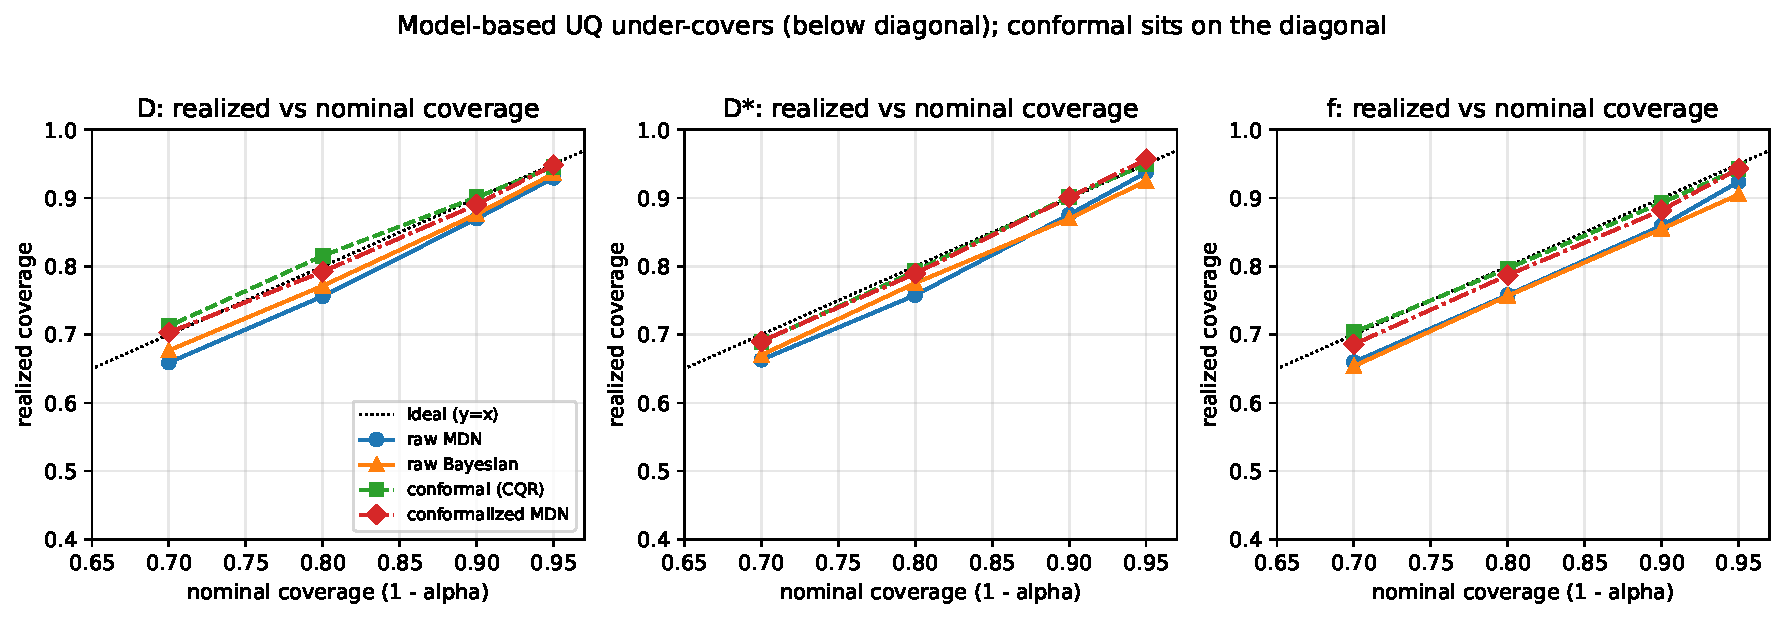
\includegraphics[width=0.78\linewidth]{figures/coverage_vs_nominal.pdf}
\caption{Realized vs nominal coverage per parameter. Raw model-based methods sit
below the diagonal (overconfident); conformal and conformalized methods sit on it.}
\label{fig:coverage}
\end{figure}

% [Fig. sharpness relocated to Supporting Information]

\subsection{The conditional finding: high-$\Dstar$ under-covers universally}
\label{sec:conditional}
Marginal coverage hides a compartment-specific failure
(Fig.~\ref{fig:heatmap}). On the (SNR $\times$ $\Dstar$-tercile) grid, the
high-$\Dstar$ tercile under-covers for \emph{every} method at \emph{every} SNR,
while the mid-$\Dstar$ tercile over-covers ($\approx0.99$). Table~\ref{tab:hidstar}
gives the high-$\Dstar$ slice: even the best method (conformalized-MDN) reaches
only $0.868$\band{0.856}{0.889} marginal-in-regime and $0.786$\band{0.751}{0.826}
in its worst-SNR cell (16-seed mean and $[5,95]$ band). Critically,
\emph{Mondrian stratification by the known SNR does not fix it} -- the failure axis
is the \emph{unknown} true $\Dstar$, not SNR. This is the refined, IVIM-specific
form of the original hypothesis.

\begin{table}[t]
\centering
\caption{High-$\Dstar$ tercile coverage ($\Dstar$ parameter, nominal $0.90$). Every
method under-covers; SNR-Mondrian does not close it. Across-seed means with 16-seed
$[5,95]$ bands. From \texttt{results/multiseed\_report.txt}.}
\label{tab:hidstar}
\small
\begin{tabular}{lcc}
\toprule
arm & hi-$\Dstar$ marginal & hi-$\Dstar$ worst-SNR cell \\
\midrule
raw-MDN              & 0.841\band{0.829}{0.857} & 0.753\band{0.719}{0.789} \\
CQR (plain)          & 0.826\band{0.809}{0.851} & 0.761\band{0.729}{0.795} \\
split (Mondrian/SNR) & 0.829\band{0.813}{0.844} & 0.781\band{0.743}{0.810} \\
CQR (Mondrian/SNR)   & 0.829\band{0.811}{0.854} & 0.789\band{0.752}{0.828} \\
conformalized-MDN    & \textbf{0.868}\band{0.856}{0.889} & \textbf{0.786}\band{0.751}{0.826} \\
\bottomrule
\end{tabular}
\end{table}

\begin{figure}[t]
\centering
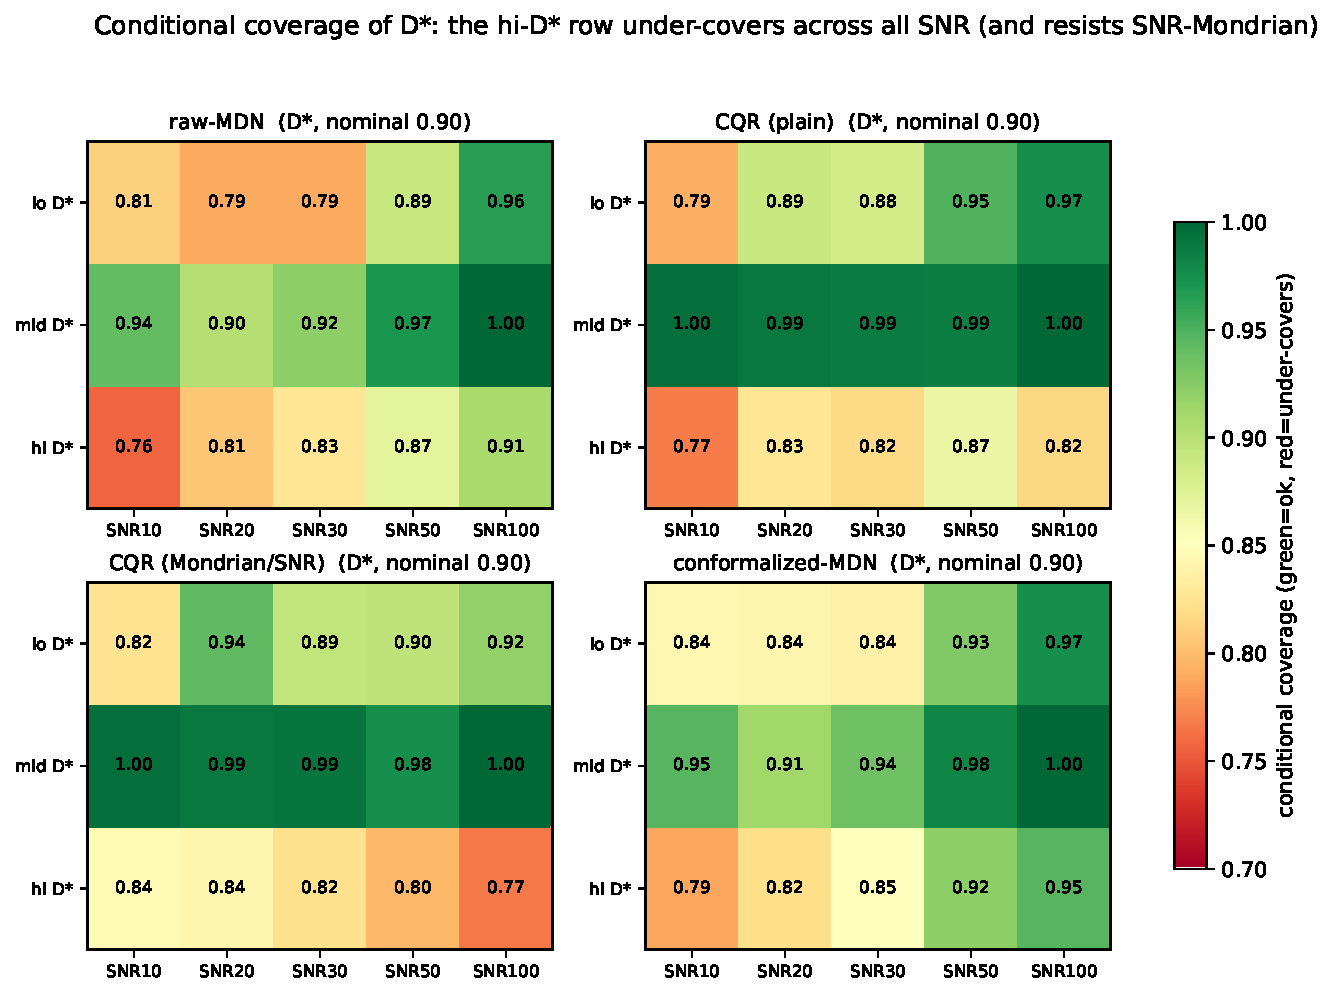
\includegraphics[width=0.72\linewidth]{figures/conditional_coverage_heatmap.pdf}
\caption{SNR $\times$ $\Dstar$-regime conditional coverage. The high-$\Dstar$ row
under-covers robustly at low-to-moderate SNR (recovering toward nominal only at the
highest SNR) and resists SNR-Mondrian.}
\label{fig:heatmap}
\end{figure}

\subsection{The high-$\Dstar$ gap is a latent-axis identifiability limit}
\label{sec:identifiability}
We attacked the high-$\Dstar$ gap with eleven \emph{label-free} conditioning
methods -- plug-in Mondrian by estimated $\hat{\Dstar}$, localized conformal on
observable features~\citep{guan2023}, and conditional conformal over an observable
basis~\citep{gibbs2023} -- none of which uses the true $\Dstar$
(Fig.~\ref{fig:attack}). \emph{None materially closes the gap.} The best label-free
method (MDN with localized conformal) reaches $0.874$\band{0.860}{0.899} marginal /
$0.807$\band{0.774}{0.845} worst-SNR, within sampling noise of the $0.786$ baseline.
The reason is structural, not
methodological:
\begin{itemize}
\item \textbf{Routing error.} A plug-in $\hat{\Dstar}$ misroutes $\sim33\%$
($[30,35]\%$ over 16 seeds) of true high-$\Dstar$ voxels to a lower-$\Dstar$
(smaller-radius) stratum: the estimate is least reliable exactly where it must
route correctly. Mondrian-by-$\hat{\Dstar}$ attains nominal coverage
\emph{conditional on the observed stratum} ($[0.90,0.89,0.90]$) yet craters on the
\emph{true} high-$\Dstar$ tercile ($0.78$\band{0.76}{0.80}) -- it controls the
observable, not the latent axis.
\item \textbf{The CRLB wall.} The CRLB on $\Dstar$ grows $\sim6\times$ from low to
high $\Dstar$ (an analytic, seed-invariant bound); the ratio of median
CRLB($\Dstar$) to the tercile bin width rises $0.34\to0.67\to1.10$ across terciles,
the high tercile band $[1.02,1.15]$ (Fig.~\ref{fig:crlb}). In the high-$\Dstar$
regime the CRLB \emph{exceeds} the bin width: a voxel's $\Dstar$ cannot be
localized to its own tercile from the data, so no observable can route it to a
wider-interval stratum. Conformal interval width correctly tracks the per-voxel
CRLB (log--log $r=0.76$\band{0.72}{0.77}): the intervals are honest, not broken.
\end{itemize}
\textbf{Verdict.} High-$\Dstar$ regime-conditional coverage in IVIM is
unrecoverable label-free for two compounding reasons. The conditioning axis (true
$\Dstar$ regime) is latent and unidentifiable, so distribution-free conditional
coverage on it is impossible~\citep{barber2021limits} -- this is the operative
barrier to coverage. Separately, $\Dstar$ is poorly point-identified there
(CRLB $\approx$ regime-bin width) -- this is why even the point map is
untrustworthy. We \emph{characterize} the limit; we do not claim to solve it.

\begin{figure}[t]
\centering

\includegraphics[width=0.82\linewidth]{figures/highdstar_attack.pdf}
\caption{High-$\Dstar$ coverage (marginal and worst-SNR cell) for eleven label-free
conditioning methods; every bar sits below the nominal $0.90$.}
\label{fig:attack}
\end{figure}

\begin{figure}[t]
\centering

\includegraphics[width=0.92\linewidth]{figures/crlb_identifiability.pdf}
\caption{(Left) absolute CRLB($\Dstar$) balloons across the $\Dstar$ range per SNR
(high-$\Dstar$ tercile shaded). (Right) conformal width vs per-voxel CRLB
($r=0.76$): the intervals widen honestly where $\Dstar$ is under-identified.}
\label{fig:crlb}
\end{figure}

\subsection{Robustness under deliberate exchangeability breaks}
\label{sec:robustness}
We deploy one conformal predictor and one monitor, calibrated on the i.i.d.\ Rician
cohort, against four deliberate breaks (Table~\ref{tab:shift},
Fig.~\ref{fig:shift}). Every break miscalibrates coverage; the dangerous
under-coverage reaches $\Dstar=0.508$\band{0.479}{0.543} under a harder-tissue prior
shift and the worst parameter $0.592$\band{0.557}{0.637} under a low-SNR covariate
shift. \emph{Weighted / nonexchangeable conformal}~\citep{tibshirani2019,barber2023}
recovers the covariate shifts (SNR worst-parameter $0.592\to0.882$, all within
$0.018$ of nominal; prior $\Dstar$ $0.508\to0.991$\band{0.974}{1.000}) and is
honestly limited on the tri-exponential forward-model misspecification: a shift in
the conditional law $P(y\mid x)$ is, in general, not repairable by an $x$-space
likelihood ratio (weighting over-corrects $\Dstar$ to $0.933$\band{0.924}{0.941},
leaving a per-parameter spread of $0.033$).

\begin{table}[t]
\centering
\caption{Per-parameter coverage under each break, naive vs.\ weighted conformal
($\alpha=0.10$, nominal $0.90$), with the deployment monitor's verdict. Across-seed
means (16 seeds); per-entry $[5,95]$ bands are in the supplementary CI table
(\texttt{results/ci\_for\_latex.json}). Monitor AUCs are the deterministic seed-0
values. From \texttt{results/multiseed\_report.txt}.}
\label{tab:shift}
\small
\begin{tabular}{llccc l}
\toprule
scenario & method & $D$ & $\Dstar$ & $f$ & monitor \\
\midrule
in-dist (control)   & naive    & 0.898 & 0.898 & 0.901 & silent (AUC 0.50) \\
SNR shift (low)      & naive    & \textbf{0.592} & 0.739 & \textbf{0.614} & FIRES (AUC 0.91) \\
                     & weighted & 0.882 & 0.901 & 0.909 & \\
prior shift (harder) & naive    & 0.972 & \textbf{0.508} & 0.909 & FIRES (AUC 0.71) \\
                     & weighted & 0.919 & 0.991 & 0.902 & \\
tri-exp misspec      & naive    & 0.907 & 0.843 & 0.912 & FIRES (AUC 0.51) \\
                     & weighted & 0.891 & 0.933 & 0.898 & \\
noise-model swap     & naive    & 0.912 & 0.893 & 0.906 & FIRES (AUC 0.52) \\
\bottomrule
\end{tabular}
\end{table}

The label-free monitor (reusing the deployment-validity concept of a sibling
project) \textbf{fires on all four observable breaks before coverage fails}: in an
SNR-severity sweep, it raises the alarm at SNR $20$ (coverage still $0.866$) while
coverage first crosses the failure line at SNR $13$. Yet it is constitutively
\emph{blind} to the latent high-$\Dstar$ gap: on an in-distribution (exchangeable)
test the monitor is silent (AUC $0.50$) and marginal $\Dstar$ coverage is nominal
($0.898$\band{0.880}{0.913}), while the high-$\Dstar$ conditional coverage is
$0.814$\band{0.787}{0.839}. Observable
shifts are caught; the within-distribution latent-axis failure is not -- the same
observable-vs-hidden split that recurs across this line of work.

% [Fig. shift relocated to Supporting Information]


\subsection{Acquisition sensitivity: the wall is b-scheme-robust}
\label{sec:acquisition}
Does the high-$\Dstar$ wall move with the b-value scheme? We compare a clinical
($11$-value), a CRLB-optimal ($11$-value, greedy $\Dstar$-CRLB design), and a dense
($22$-value) scheme at fixed prior/SNR/seed (Table~\ref{tab:acq},
Fig.~\ref{fig:acq}). The high-$\Dstar$ marginal coverage barely moves
($0.821\to0.835\to0.808$). The resolution ratio CRLB($\Dstar$)/tercile-width stays
at or above unity: even a CRLB-optimal design only reaches $\sim$unity
($1.03$\band{0.97}{1.16}); acquisition shifts the wall to threshold, not past it,
while the clinical and dense schemes stay above it ($1.24$, $1.11$). A CRLB-optimal
design lowers the ratio ($1.24\to1.03$) but does not remove the wall. Acquisition
design \emph{shifts} the wall; it does not erase it -- a concrete, honestly negative
handoff to acquisition-aware experiment design.

\begin{table}[t]
\centering
\caption{High-$\Dstar$ coverage and resolution ratio by b-value scheme. Across-seed
means with 16-seed $[5,95]$ bands; the CRLB-optimal ratio band crosses unity. From
\texttt{results/multiseed\_report.txt}.}
\label{tab:acq}
\small
\begin{tabular}{lcccc}
\toprule
scheme & $n_b$ & hi-$\Dstar$ marg & hi-$\Dstar$ worst-SNR & CRLB/tercile-width \\
\midrule
clinical      & 11 & 0.821\band{0.794}{0.845} & 0.596\band{0.542}{0.702} & 1.24\band{1.17}{1.37} \\
CRLB-optimal  & 11 & 0.835\band{0.795}{0.862} & 0.603\band{0.541}{0.678} & \textbf{1.03}\band{0.97}{1.16} \\
dense         & 22 & 0.808\band{0.788}{0.836} & 0.551\band{0.508}{0.597} & 1.11\band{1.05}{1.21} \\
\bottomrule
\end{tabular}
\end{table}

\begin{figure}[t]
\centering
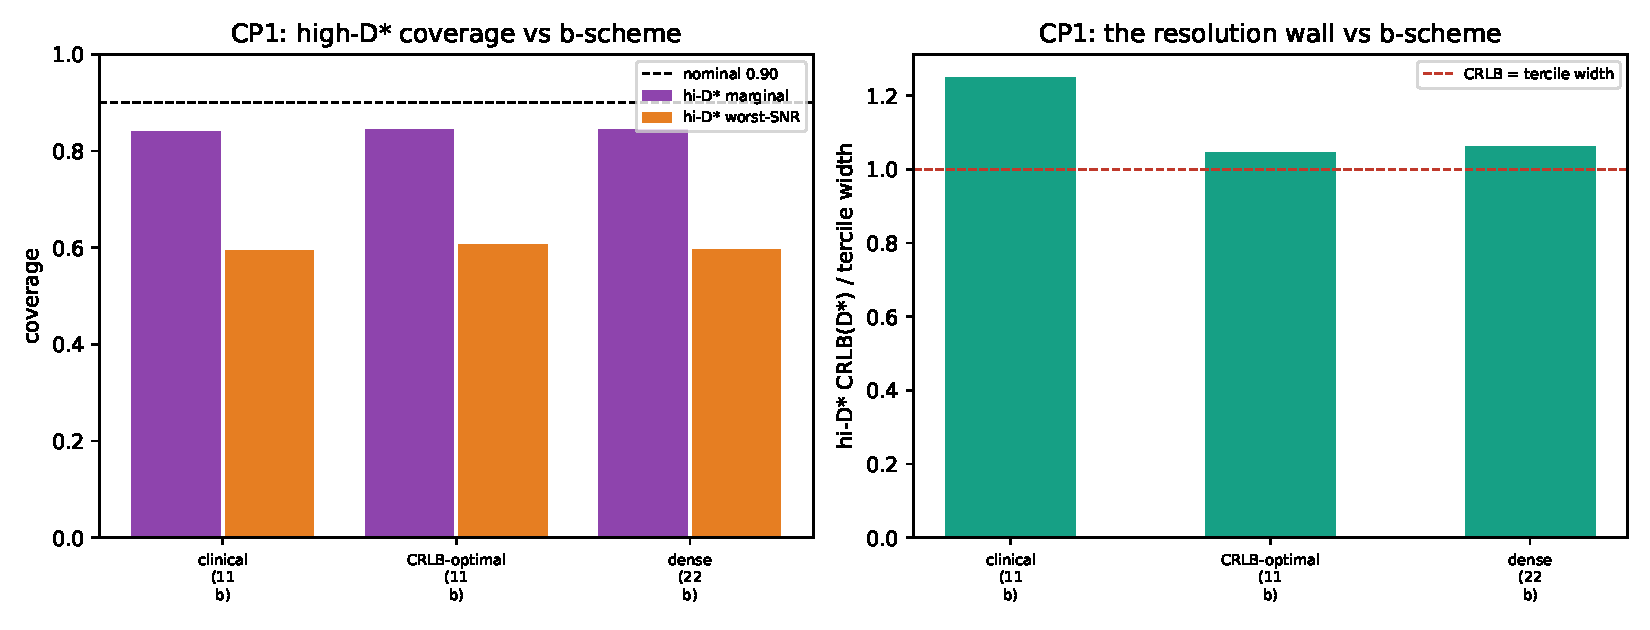
\includegraphics[width=0.92\linewidth]{figures/acquisition_wall.pdf}
\caption{(Left) high-$\Dstar$ coverage vs.\ b-scheme. (Right) the resolution ratio
CRLB($\Dstar$)/tercile-width stays at or above unity for every scheme (the
CRLB-optimal band dips to $0.97$): acquisition moves the regime to the resolution
threshold, not past it.}
\label{fig:acq}
\end{figure}

\subsection{In-vivo: a qualitative demonstration, no coverage claim}
\label{sec:invivo}
In vivo there are no ground-truth parameters, so realized coverage is
\emph{unmeasurable} and the finite-sample guarantee is \emph{not asserted}. We
demonstrate the deployed pipeline qualitatively (Fig.~\ref{fig:invivo}): the
conformalized $\Dstar$ band widths are wide and heavy-tailed ($10/50/90$th
percentile $=47/64/79\times10^{-3}\unit{mm^2/s}$; widest-to-narrowest decile ratio
$1.7\times$), ballooning on voxels where the perfusion compartment is
under-identified -- the wall, now on signal. Pointed at the deployment data with a
synthetic calibration, the deployment monitor \textbf{fires} (AUC $0.84$):
synthetic$\to$deployment is itself a large exchangeability break, and the monitor
detects it. That firing is the honest, label-free reason the synthetic guarantee
must not be transferred in vivo without re-calibration on matched labeled data --
which in vivo does not exist. The monitor turns ``no ground truth'' into an
observable stop sign. The demonstration above uses a clearly labeled synthetic
stand-in; Sec.~\ref{sec:invivo-real} repeats the \emph{as-deployed} pipeline on a
real, permissively-licensed in-vivo collection, where the monitor fires on the
synthetic$\to$real transfer for the same reason.

% [Fig. synthetic in-vivo demo relocated to Supporting Information]


\subsection{Real in-vivo data: the same pipeline, the monitor fires on transfer}
\label{sec:invivo-real}
We additionally run the as-deployed pipeline on real multi-$b$ in-vivo DWI from the
public ACRIN-6698 / I-SPY2 Breast DWI collection (The Cancer Imaging Archive;
CC-BY-4.0)~\cite{acrin6698,clark2013tcia}, retrieved on demand (no pixel data are
redistributed with this work). This is a 4-$b$ ADC protocol
($b=\{0,100,600,800\}\unit{s/mm^2}$), \emph{not} IVIM-optimized, with no
ground-truth IVIM parameters; it therefore supports only qualitative
pipeline/monitor behavior and makes \textbf{no in-vivo coverage claim}. A predictor
trained on the synthetic 22-value scheme cannot ingest a 4-$b$ signal, and
interpolation would fabricate unacquired $b$-values, so we keep the deployment
\emph{monitor} as-deployed---its observable features are $b$-independent---and
re-fit only the CQR band at the real 4-$b$ scheme; the resulting bands are
qualitative, not coverage intervals.

Figure~\ref{fig:invivo-maps} shows the actual images on a representative slice: the
real $b{=}0$ breast DWI, the plug-in $\hat{\Dstar}$ map, and the per-voxel conformal
$\Dstar$ band-width (uncertainty) map, with the whole-tumor ROI outlined. The
uncertainty map is spatially heterogeneous and widens exactly where the perfusion
compartment is under-identified---the identifiability wall, now visible on real
tissue.

\begin{figure}[t]
\centering

\includegraphics[width=\linewidth]{figures/invivo_real_maps.pdf}
\caption{Actual in-vivo images (ACRIN-6698 / I-SPY2 Breast DWI; one slice;
qualitative, no coverage claim). (Left) real $b{=}0$ DWI with the whole-tumor ROI in
red; (middle) the plug-in $\hat{\Dstar}$ perfusion map; (right) the per-voxel
conformal $\Dstar$ band-width map---wider where the perfusion compartment is
under-identified. The synthetic 22-value-calibrated monitor (not shown here) fires
on this data; see Fig.~\ref{fig:invivo-real}.}
\label{fig:invivo-maps}
\end{figure}

On $4000$ foreground voxels the as-deployed monitor \textbf{fires} (AUC $0.97$) and
the $\Dstar$ band stays wide ($10/50/90$th percentile
$=64/79/86\times10^{-3}\unit{mm^2/s}$; Fig.~\ref{fig:invivo-real}). The firing is
carried entirely by the $b$-independent Mahalanobis family (Family-1); the residual
family (Family-2) is silent because a 4-$b$ acquisition exactly-determines the
four-parameter IVIM fit, collapsing the fit-residual norm to zero. The monitor has
therefore \emph{not} half-failed---it has localized the break to the feature
distribution. The sparse-protocol-plus-real-tissue gap is a large exchangeability
break, which is exactly why the synthetic guarantee \emph{correctly refuses} to
transfer.

\paragraph{Test--retest repeatability.}
ACRIN-6698 includes a same-day test--retest arm: two coffee-break repeat DWI exams
acquired in a single visit (tagged \texttt{TrT0}/\texttt{TrT1}), which we use here.
(This genuine same-visit arm supersedes an earlier $n{=}11$ pairing that had
inadvertently matched \emph{longitudinal} timepoints months apart, confounded by
interval treatment.) Across $n{=}76$ tumors we ask, label-free, whether the
conformal interval width \emph{tracks} the scan--rescan variability of the plug-in
estimate (region-level over the whole-tumor ROI; the two repeats are unregistered,
so this is not a per-voxel statement). The identifiability wall makes a directional
prediction we fix before looking: the interval width should track measured
scan--rescan repeatability for the well-identified diffusion compartment $D$, and
should track it weakly or not at all for $\Dstar$, whose regime the data cannot
resolve. A positive $\Dstar$ association would count against the wall. For the
well-identified tissue diffusion $D$,
the conformal $D$-width is associated with the measured scan--rescan
$|\Delta\mathrm{ADC}|$ (Spearman $r=+0.60$, $p<0.001$, 95\% CI $[0.42,0.72]$ by
BCa bootstrap): the interval \emph{widens where the real measurement is least
repeatable}. At $n{=}76$ the association is now \textbf{robust} (the CI excludes
zero, versus the wide interval at the earlier $n{=}11$), and stable across field
strength (1.5\,T $r{=}{+}0.58$, $n{=}49$; 3.0\,T $r{=}{+}0.50$, $n{=}27$) and
pretreatment-only ($r{=}{+}0.61$, $n{=}65$). For $\Dstar$ the association is not
significant ($r=-0.17$, $p=0.13$, 95\% CI $[-0.39,0.05]$ spanning zero), matching
the pre-stated prediction: the association holds for the parameter the data
identify ($D$) and is absent for the one they do not ($\Dstar$). The $\Dstar$ null
is the predicted outcome, not a post-hoc reading. This is a
repeatability-tracking check, \emph{not} a statement of validation, accuracy,
calibration, or coverage.

\begin{figure}[t]
\centering

\includegraphics[width=0.92\linewidth]{figures/invivo_real_demo.pdf}\\[2pt]

\includegraphics[width=0.55\linewidth]{figures/invivo_real_retest.pdf}
\caption{Real in-vivo data (ACRIN-6698 / I-SPY2 Breast DWI; qualitative, no coverage
claim). (Top left) the re-fit conformal $\Dstar$ band vs the plug-in $\hat{\Dstar}$;
(top right) the $\Dstar$ band-width distribution and the as-deployed monitor verdict
(fires, AUC $0.97$, via the $b$-independent Mahalanobis family). (Bottom)
test--retest: the conformal $D$-width vs the measured scan--rescan ADC variability
across $n{=}76$ same-day-repeat tumors (Spearman $r=+0.60$, 95\% CI $[0.42,0.72]$;
robust, repeatability-tracking only---not validation or coverage).}
\label{fig:invivo-real}
\end{figure}

\subsection{External-phantom replication on the OSIPI IVIM reference}
\label{sec:osipi}
Every coverage number above is, by necessity, computed on \emph{our} labeled
synthetic cohort -- our forward model and our parameter prior. To neutralise the
``validated only on the authors' own forward model'' concern on the part that
matters, we replicate the coverage results and the high-$\Dstar$ wall against an
\textbf{external, community-standard \emph{synthetic} reference}: the OSIPI
(ISMRM Open Science Initiative for Perfusion Imaging) TF2.4 IVIM digital reference
object (DRO), $5000$ voxels with ground-truth $(D,\Dstar,f)$ that \emph{we did not
generate}~\citep{osipi_ivim} (Zenodo \texttt{doi:10.5281/zenodo.14605039},
CC-BY-4.0; fetched on demand, provenance only committed). This is an
\emph{independent synthetic} reference, \textbf{not} in vivo: in-vivo coverage
validation remains structurally impossible (no ground truth), so no in-vivo
coverage claim is made here. The bi-exponential signal model is the field's
consensus model and is therefore shared by construction; what is external is the
ground-truth \emph{parameter distribution}. That distribution is genuinely shifted
from ours: the OSIPI true $\Dstar$ spans $\sim\!0.05$--$0.20\,\mathrm{mm^2/s}$,
above our calibration prior ($0.01$--$0.10$), so transferring our calibration onto
it is a real out-of-distribution test. All numbers are across-seed means with
$[5,95]$ bands over $16$ seeds; nominal coverage is $0.90$.

We evaluate two regimes -- \emph{controlled} (OSIPI ground truth, re-synthesised at
\emph{our} 22-$b$ acquisition and SNR grid, so only the parameter distribution is
swapped) and \emph{native} (the DRO's own pre-noised signals at its native sparse
7-$b$ scheme) -- each under \emph{naive transfer} (calibrate on our synthetic
cohort, test on OSIPI) and \emph{recalibrated} (split the OSIPI DRO and calibrate
within its distribution). Table~\ref{tab:osipi} gives the marginal coverage and the
top-$\Dstar$-tercile conditional coverage; Fig.~\ref{fig:osipi} plots them with the
wall metric.

\begin{table}[t]
\centering\small
\begin{tabular}{llcccc}
\toprule
regime & calibration & $D$ & $\Dstar$ & $f$ & hi-$\Dstar$ tercile \\
\midrule
controlled & naive transfer & 0.597\band{0.567}{0.621} & 0.304\band{0.285}{0.315} & 0.495\band{0.472}{0.512} & 0.000\band{0.000}{0.000} \\
controlled & recalibrated   & 0.899\band{0.881}{0.913} & 0.905\band{0.889}{0.921} & 0.904\band{0.892}{0.919} & 0.823\band{0.786}{0.853} \\
native     & naive transfer & 0.693\band{0.643}{0.758} & 0.291\band{0.263}{0.312} & 0.524\band{0.497}{0.542} & 0.000\band{0.000}{0.000} \\
native     & recalibrated   & 0.898\band{0.888}{0.913} & 0.899\band{0.884}{0.909} & 0.894\band{0.882}{0.908} & 0.831\band{0.798}{0.869} \\
\bottomrule
\end{tabular}
\caption{Conformal/CQR coverage on the OSIPI external \emph{synthetic} DRO at
nominal $0.90$ (CQR; across-seed mean over $16$ seeds, $[5,95]$ band). \emph{Naive
transfer} of our synthetic calibration breaks under the real $\Dstar$ distribution
shift; \emph{recalibrating} within the OSIPI distribution restores marginal coverage
to nominal on independent ground truth, yet the high-$\Dstar$ conditional coverage
stays below nominal -- the identifiability wall, on data we did not generate.}
\label{tab:osipi}
\end{table}

\paragraph{Naive transfer breaks, and the monitor says so.} Transferring our
synthetic calibration onto the OSIPI ground truth breaks marginal coverage
(controlled $\Dstar$ $0.304$\band{0.285}{0.315}, $D$ $0.597$\band{0.567}{0.621}),
exactly as the exchangeability theory predicts for a real distribution shift.
Critically, the label-free deployment monitor \emph{fires on every one of the $16$
seeds} (Mahalanobis AUC $0.737$\band{0.726}{0.750}, controlled): the shift is
observable, so the monitor correctly refuses the transfer. As in the sparse-protocol
in-vivo case (\S\ref{sec:invivo-real}), a fired monitor here is the system working,
not failing.

\paragraph{Recalibrated coverage holds on independent ground truth.} Splitting the
OSIPI DRO and recalibrating within its own distribution restores marginal coverage
to nominal for all three parameters ($D$ $0.899$\band{0.881}{0.913}, $\Dstar$
$0.905$\band{0.889}{0.921}, $f$ $0.904$\band{0.892}{0.919}; native nearly
identical) -- the finite-sample conformal guarantee transfers cleanly to a forward
model and parameter distribution we did not author.

\paragraph{The high-$\Dstar$ wall replicates -- it is information, not our model.}
Even after within-distribution recalibration, coverage conditional on the true
$\Dstar$ tercile craters in the high-$\Dstar$ regime ($0.823$\band{0.786}{0.853}
controlled, $0.831$\band{0.798}{0.869} native) while the low-$\Dstar$ tercile sits
at nominal ($0.899$\band{0.859}{0.931}). On the OSIPI ground truth at our
acquisition the CRLB$(\Dstar)$/tercile-width ratio rises $0.46\!\to\!0.86\!\to\!1.53$
(\band{1.407}{1.753} at high $\Dstar$) with the absolute CRLB growing
$3.5\times$\band{3.1}{4.0} -- the same wall as Fig.~\ref{fig:crlb}, on a digital
reference object we did not build. This regime also dissociates the two mechanisms
directly: in the native high-SNR setting the CRLB ratio stays below $1$, yet the
conditional gap persists. The coverage failure therefore survives where the CRLB
does \emph{not} exceed the bin width, so it is driven by conditioning on a latent
axis the data do not identify~\citep{barber2021limits}, not by CRLB magnitude. CRLB
magnitude governs point-identifiability; latent conditioning governs label-free
coverage. That the wall reproduces on an external
ground truth is strong evidence it is information-theoretic, intrinsic to the
perfusion-estimation problem and the data -- it replicates even when the ground
truth is generated by a non-bi-exponential, velocity-dispersion mechanism
(Sec.~\ref{sec:altmodel}) -- rather than an artifact of our particular
forward model or prior.

\begin{figure}[t]
\centering
\includegraphics[width=\linewidth]{figures/osipi_coverage.pdf}
\caption{OSIPI external \emph{synthetic} reference (DRO; not in vivo, no in-vivo
coverage claim). (A) Marginal coverage vs nominal: naive transfer of our synthetic
calibration breaks, recalibrating within the OSIPI distribution restores it. (B)
Coverage conditional on the true $\Dstar$ tercile: the high-$\Dstar$ gap persists
even after recalibration. (C) The identifiability wall on OSIPI ground truth --
CRLB$(\Dstar)$ exceeds the high-$\Dstar$ tercile width. The naive-transfer monitor
fires (AUC $0.74$), so the break is flagged.}
\label{fig:osipi}
\end{figure}

\subsection{Point accuracy does not buy conditional coverage: a deliberately
biased estimator}
\label{sec:dissociation-shrinkage}
A natural objection to the identifiability reading (Sec.~\ref{sec:identifiability})
is that the unbiased baselines merely leave precision on the table: a \emph{biased},
prior-shrinkage Bayesian fit was historically the one IVIM estimator that kept
$\Dstar$ variance under control where unbiased fits failed, and a biased estimator
can legitimately sit below the \emph{unbiased} Cram\'er--Rao
bound~\citep{gurneychampion2018}. If the high-$\Dstar$ wall were a point-precision
artifact, such an estimator should breach it. We pushed a deliberately biased,
label-free shrinkage prior (a fixed log-normal $\Dstar$/$f$ prior with the
NLLS-residual noise scale -- it uses no labels) through the same
conditional-coverage machinery (Table~\ref{tab:dissociation}).

The prior behaves as a shrinkage prior should: it lowers $\Dstar$ point RMSE in the
low tercile ($15.1$\band{14.7}{15.6} vs.\ the unbiased MCMC's
$17.8$\band{17.2}{18.5}, in $10^{-3}$\,mm$^2$/s) by trading variance for a
centre-pulling bias. But in the deciding high-$\Dstar$ tercile that bias dominates:
point RMSE does \emph{not} improve ($24.6$\band{24.1}{25.3} vs.\
$20.5$\band{19.9}{21.1}), carried by a large negative bias
($-18.8$\band{-19.2}{-18.3} vs.\ $-14.2$\band{-14.5}{-13.7}) from pulling
high-$\Dstar$ voxels toward the cohort centre. Crucially, high-$\Dstar$
regime-conditional coverage does not rise: the conformalized marginal
$0.827$\band{0.801}{0.845} and worst-SNR cell $0.721$\band{0.663}{0.765} sit at or
below the unbiased arms ($0.889$\band{0.872}{0.903} / $0.857$\band{0.826}{0.875} for
MCMC), nowhere near nominal $0.90$. Two pre-registered sanity gates exclude the
artifactual readings: the shrinkage interval does \emph{not} collapse (median
high-$\Dstar$ width $55.0$\band{53.6}{56.6} vs.\ comparator $47.9$, in
$10^{-3}$; $1.15\times$), and the estimator's own point still misroutes
$34$\band{32}{36}\% of true-high-$\Dstar$ voxels (the NLLS plug-in misroutes
$\sim33\%$), so any coverage change would have to arise \emph{despite} routing, not
by repairing it. Trading variance for bias buys point precision in the identified
terciles but not conditional coverage where the conditioning axis is latent:
consistent with the identifiability reading, the barrier is information, not point
precision. The argument is mechanism-level -- any centre-pulling bias trades
variance for bias, and in the high-$\Dstar$ tercile the bias dominates -- so it
brackets the historically $\Dstar$-stabilizing prior-shrinkage Bayesian
fit~\citep{gurneychampion2018} rather than hinging on one prior choice. This
strengthens the claim within its scope -- it now holds even for a
deliberately biased prior-shrinkage method -- but remains a statement about the
label-free methods we tested, not about any conceivable estimator.

\begin{table}[t]
\centering
\caption{Point-accuracy / conditional-coverage \emph{dissociation} for a
deliberately biased shrinkage prior. RMSE and bias in $10^{-3}$\,mm$^2$/s; coverage
of the conformalized $\Dstar$ band (nominal $0.90$). Across-seed means with 16-seed
$[5,95]$ bands. From \texttt{results/multiseed\_report.txt} /
\texttt{results/dissociation\_report.txt}.}
\label{tab:dissociation}
\small
\begin{tabular}{lcccc}
\toprule
arm & hi-$\Dstar$ RMSE & hi-$\Dstar$ bias & hi-$\Dstar$ marginal & hi-$\Dstar$ worst-SNR \\
\midrule
Bayesian-shrinkage & 24.6\band{24.1}{25.3} & $-18.8$\band{-19.2}{-18.3} & 0.827\band{0.801}{0.845} & 0.721\band{0.663}{0.765} \\
Bayesian-MCMC      & \textbf{20.5}\band{19.9}{21.1} & $-14.2$\band{-14.5}{-13.7} & \textbf{0.889}\band{0.872}{0.903} & \textbf{0.857}\band{0.826}{0.875} \\
conformalized-MDN  & 20.3\band{19.6}{21.0} & $-13.4$\band{-14.2}{-12.8} & 0.867\band{0.853}{0.884} & 0.784\band{0.742}{0.819} \\
\bottomrule
\end{tabular}
\end{table}

\subsection{The wall replicates under a non-bi-exponential generator}
\label{sec:altmodel}
The external-phantom replication (Sec.~\ref{sec:osipi}) still draws its ground truth
from a bi-exponential model. To test whether the high-$\Dstar$ wall is an artifact
of Eq.~\eqref{eq:ivim} itself, we regenerate the cohort from a genuinely
\emph{non}-bi-exponential mechanism: a gamma velocity-dispersion perfusion process
(coefficient of variation $0.5$, shape $k=4$) whose signal is \emph{not} a
realization of Eq.~\eqref{eq:ivim}. Because such a signal has no single ``true''
$\Dstar$, we report the effective pseudo-diffusion $\Dstar_{\mathrm{eff}}$ on two
axes: a primary, non-circular axis (A) the analytic perfusion log-slope (the gamma
mean, defined without reference to a bi-exponential fit) and a corroborating axis
(B) the best-fit bi-exponential $\Dstar$. The non-circularity of the test rests on
axis A; axis B, which defines the regime by fitting Eq.~\eqref{eq:ivim} to signals
Eq.~\eqref{eq:ivim} did not generate, is reported only to confirm the two
definitions agree. Calibration and recalibration use the OSIPI
within-distribution harness (Sec.~\ref{sec:osipi}).

After recalibrating \emph{within} the dispersion distribution, marginal coverage is
restored ($\Dstar_{\mathrm{eff}}$ marginal $0.898$\band{0.880}{0.917} on axis A),
yet the high-$\Dstar_{\mathrm{eff}}$ tercile-conditional coverage stays well below
nominal on both axes -- $0.796$\band{0.748}{0.854} (A) and $0.800$\band{0.756}{0.845}
(B) (Fig.~\ref{fig:altmodel}A), a gap of $\sim0.10$ that the bi-exponential CRLB
cannot have caused because the
generator is not bi-exponential. The wall is therefore a property of the
perfusion-estimation problem more broadly, not of our forward model: it survives a
generator that Eq.~\eqref{eq:ivim} does not even contain. A second dispersion kernel
(log-normal, same CV) reproduces the effect (high-$\Dstar_{\mathrm{eff}}$
$0.797$\band{0.747}{0.847}), so it is not specific to the gamma parametrization. A
continuity gate confirms the construction is sound: at zero dispersion the generator
reduces to the bi-exponential cohort exactly (max
$|S_{\mathrm{disp}}(\mathrm{CV}{=}0)-S_{\mathrm{biexp}}|=0.00\mathrm{e}{+}00$,
numerically exact), and its recalibrated high-$\Dstar$ coverage there
($0.798$\band{0.750}{0.842}) lands on the bi-exponential wall -- the dispersion
cohort contains the bi-exponential model as its zero-deviation limit. Consistent
with the observable-vs-latent reading (Sec.~\ref{sec:identifiability}), this
forward-model misspecification is largely a \emph{hidden} channel: the naive-transfer
deployment monitor barely separates the dispersion cohort from the bi-exponential
calibration (AUC $0.501$\band{0.481}{0.519}, at chance), so the break is one the
monitor cannot, by construction, see.

\subsection{The off-model validity envelope}
\label{sec:envelope}
The tri-exponential stress in Sec.~\ref{sec:robustness} is a single off-model probe.
We replace it with a \emph{validity envelope}: holding the deployed,
bi-exponential-calibrated predictor fixed, we sweep three independent deviation
families -- velocity dispersion (CV up to $0.8$), a tri-exponential third
compartment (weight up to $0.4$), and a stretched-exponential signal ($|1-\beta|$ up
to $0.6$) -- and trace how coverage degrades and whether the monitor tracks the drift
(Fig.~\ref{fig:altmodel}B,C). Marginal coverage degrades gracefully and
monotonically with deviation: by the largest deviation, $\Dstar$ coverage falls to
$0.769$\band{0.736}{0.788} (tri-exponential) and $0.770$\band{0.749}{0.793}
(stretched), and perfusion-fraction coverage to $0.791$\band{0.767}{0.815}
(dispersion). The envelope contains the bi-exponential model as its origin: at zero
deviation coverage recovers to nominal ($\Dstar$ $0.903$\band{0.880}{0.918}). The
deployment monitor's discrimination of off-model drift is real but weak and
family-dependent -- its AUC rises with deviation for the tri-exponential family
($0.532$\band{0.515}{0.548} at the largest step) yet stays near chance for pure
velocity dispersion -- so although the cohort-level alarm fires at or before the
deviation at which marginal coverage first fails, off-model misspecification is only
partly observable, reinforcing that some forward-model breaks are hidden channels
(Sec.~\ref{sec:altmodel}). The single tri-exponential number thus generalizes to a
characterized envelope: a known, monitored degradation rate with a recovered
bi-exponential origin, rather than one probe.

\begin{figure}[t]
\centering

\includegraphics[width=\linewidth]{figures/altmodel.pdf}
\caption{Alternative forward model. (A) Arm~1 -- $\Dstar_{\mathrm{eff}}$-tercile
conditional coverage when the ground truth is a non-bi-exponential velocity-dispersion
process: after within-distribution recalibration the high-$\Dstar_{\mathrm{eff}}$
gap persists on both surrogate axes (primary gamma mean A, corroborating bi-exp-fit B), while naive
transfer breaks. (B) Arm~2 -- marginal $\Dstar$ coverage degrades monotonically as
the forward model deviates from bi-exponential across three families, recovering to
nominal at zero deviation. (C) Arm~2 -- the deployment monitor's AUC vs.\ deviation:
discrimination of off-model drift is weak and family-dependent. Across-seed means
(16 seeds); from \texttt{results/altmodel\_report.txt}.}
\label{fig:altmodel}
\end{figure}

\subsection{A clinically realistic cohort: correlated prior and measurement nuisance}
\label{sec:realism}
The cohort so far draws $(D,\Dstar,f)$ uniformly over published ranges with clean
Rician noise. As a capstone robustness check we replace both idealizations at once:
a clinically realistic \emph{joint} prior -- correlated, right-skewed marginals
(log-normal $D,\Dstar$; logit-normal $f$) with a within-subject $\Dstar$
coefficient of variation in the published $50$--$110\%$ band, shaped to
representative abdominal IVIM distributions -- and a measurement-level nuisance
layer on the bi-exponential signal under a single magnitude scalar $\eta$:
partial-volume mixing of a free-fluid compartment, bulk-motion phase, and
non-Rician (multi-coil noncentral-$\chi$) noise. This is still a synthetic cohort
and makes no in-vivo coverage claim; a continuity gate confirms the construction
reduces to the existing cohort exactly at the uniform prior with $\eta=0$ (max
$|\cdot|=0.00\mathrm{e}{+}00$, numerically exact). Because a skewed prior moves the
tercile boundaries, we report the high-$\Dstar$ regime on two stratifications: the
\emph{fixed} physical boundaries inherited from the uniform cohort -- so ``high
$\Dstar$'' denotes the same physical regime across priors (primary) -- and the
per-distribution quantiles (secondary), with the clinical prevalence of the fixed
high-$\Dstar$ bin reported so a rare regime is never mistaken for a vanished wall.

Under the realistic prior with clean acquisition (Arm~A), recalibrating
\emph{within} the distribution restores marginal coverage to nominal ($D/\Dstar/f =
0.903$\band{0.896}{0.913}, $0.900$\band{0.884}{0.917}, $0.898$\band{0.885}{0.912}),
while naive transfer of the uniform-calibrated predictor breaks ($\Dstar$ marginal
$0.767$\band{0.735}{0.805}). The high-$\Dstar$ wall persists after recalibration in
\emph{both} stratifications -- fixed-edge tercile coverage $0.533$\band{0.480}{0.594}
and per-distribution $0.786$\band{0.749}{0.823}, against nominal $0.90$ -- with the
fixed-edge CRLB-to-bin-width ratio reaching $0.895$\band{0.849}{0.961} at high
$\Dstar$ (Fig.~\ref{fig:realism}A,B). The severest under-coverage concentrates in a
clinically \emph{rare} high-$\Dstar$ tail (fixed high-$\Dstar$ prevalence
$0.049$\band{0.044}{0.056}): under a liver-like prior the ill-posed regime is
sparsely populated -- a scoping caveat we report as such, not as a weakened wall.
The realistic prior is a within-support covariate shift, so the label-free monitor
does not flag it (naive-transfer AUC $0.480$\band{0.470}{0.494}, at chance);
recalibration, not monitoring, is what restores coverage.

Holding the deployed predictor fixed and sweeping the nuisance magnitude (Arm~B),
marginal coverage degrades monotonically: $D$ coverage falls from
$0.903$\band{0.889}{0.912} at $\eta=0$ to $0.570$\band{0.548}{0.589} at $\eta=1$,
while the already-wide $\Dstar$ interval stays near nominal
($0.899$\band{0.888}{0.911}), and recalibrating within the nuisance-laden
distribution restores it ($\Dstar$ $0.899$\band{0.886}{0.914} at $\eta=1$).
Notably, this acquisition nuisance is \emph{not} more observable than pure
signal-model drift: the monitor's AUC stays at chance across the sweep
($0.493$\band{0.482}{0.507} at $\eta=1$, cf.\ the off-model envelope's
$\le0.53$), so a measurement nuisance that substantially breaks coverage is a
largely \emph{silent} channel -- again locating the operative safeguard in
recalibration rather than the observable monitor.

\begin{figure}[t]
\centering

\includegraphics[width=\linewidth]{figures/realism_cohort.pdf}
\caption{Realism cohort (realistic synthetic; no in-vivo coverage claim).
(A)~Arm~A -- marginal coverage under a realistic correlated/skewed prior: naive
transfer of the uniform-calibrated predictor breaks, within-distribution
recalibration restores nominal coverage. (B)~Arm~A -- recalibrated high-$\Dstar$
tercile coverage on fixed physical boundaries vs.\ per-distribution quantiles; the
wall persists in both, concentrated in a clinically rare high-$\Dstar$ tail (fixed
prevalence $\approx0.05$). (C)~Arm~B -- the measurement-nuisance envelope: marginal
$D$ coverage degrades with the nuisance magnitude (the wider $\Dstar$ interval is
held) while the deployment monitor's AUC stays at chance, a silent channel.
Seed-\texttt{20260613} panel (across-seed [5,95] bands quoted in text); from
\texttt{results/realism\_report.txt}.}
\label{fig:realism}
\end{figure}

\section{Discussion}
The thread connecting these results is an \emph{observable-vs-latent} distinction.
Conformal prediction guarantees \emph{marginal} coverage and, with weighting or
stratification on \emph{observable} quantities (SNR, signal features, estimated
density ratios), can recover coverage conditional on those observables. What it
cannot label-free-guarantee is coverage conditional on a \emph{latent} axis that
the data do not identify. In IVIM that latent axis is the true $\Dstar$ in its
ill-posed regime: the Fisher information there collapses, the CRLB exceeds the bin
width, and no observable proxy -- including the plug-in $\hat{\Dstar}$ -- recovers
the regime. This is why an observable deployment monitor catches every
\emph{distribution} shift but is blind to the \emph{within-distribution} high-$\Dstar$
gap. Four independent stresses corroborate that this split is information, not an
artifact of our estimator or generator: a deliberately biased shrinkage prior buys
$\Dstar$ point precision but not high-$\Dstar$ conditional coverage
(Sec.~\ref{sec:dissociation-shrinkage}); the gap replicates when the ground truth is
a non-bi-exponential velocity-dispersion process, a forward-model break that is
itself a hidden channel the monitor cannot see (Sec.~\ref{sec:altmodel}); the
off-model validity envelope degrades gracefully with a recovered bi-exponential
origin (Sec.~\ref{sec:envelope}); and the wall persists under a clinically realistic
correlated, skewed prior with measurement-level nuisance, where it concentrates in a
clinically rare high-$\Dstar$ tail and the nuisance proves a silent channel the
monitor does not see (Sec.~\ref{sec:realism}).

The same wall appears in adjacent label-free problems: deployment-validity
monitoring is provably blind to shifts that leave observable statistics unchanged
(a ``hidden channel''), and the absence of in-vivo ground truth (the ``Echo
tension'') forecloses any direct coverage check on real data. We read these not as
failures of conformal prediction -- whose guarantee is exactly as advertised -- but
as the IVIM instance of a known boundary~\citep{barber2021limits}:
distribution-free tools deliver everything the data identify and nothing they do
not. On what this delivers, stated plainly: the finite-sample coverage guarantee is
a property of the synthetic calibration and transfers in vivo only under an
exchangeability assumption that cannot be verified where no ground truth exists --
it is not an in-vivo coverage claim. What the method adds over the existing IVIM
repeatability literature is mechanistic and operational, not a usable per-voxel
in-vivo interval: (i) conformalizing a strong model-based base gives the sharpest
valid intervals on synthetic data; (ii) an observable monitor guards exchangeability
at deployment, while remaining blind to the latent high-$\Dstar$ gap by
construction; and (iii) the high-$\Dstar$ compartment is reported as
characterized-but-unresolved, with a per-voxel reason -- the identifiability wall --
rather than a trusted point map.

\section{Limitations}
Our coverage results are \emph{synthetic-primary} by necessity: conformal
calibration needs labels that in-vivo IVIM lacks, so the guarantee is established
on a forward model we control, and the in-vivo component is explicitly qualitative
with no coverage claim. We stress that this is a structural impossibility, not a
study limitation removable with more data: because in-vivo IVIM admits no
ground-truth $(D,\Dstar,f)$, realized coverage is unmeasurable in vivo in
principle, so a distribution-free coverage guarantee can only ever be
synthetic-established and then transported under an explicitly monitored
exchangeability assumption -- precisely what the real-data section
(Sec.~\ref{sec:invivo-real}) exercises, rather than a coverage claim it could never
support. The base synthetic cohort uses uniform priors over published
ranges and Rician noise; real tissue is more heterogeneous. We address this directly
with a capstone realism cohort (Sec.~\ref{sec:realism}) that draws a correlated,
right-skewed joint prior with a published-range $\Dstar$ coefficient of variation and
adds measurement-level nuisance (partial-volume mixing, bulk-motion phase, non-Rician
multi-coil noise): the marginal guarantee returns on recalibration and the
high-$\Dstar$ wall persists, concentrated in a clinically rare high-$\Dstar$ tail.
The off-model behavior is likewise characterized rather than probed at a single
point: the high-$\Dstar$ wall replicates under a non-bi-exponential
velocity-dispersion generator (Sec.~\ref{sec:altmodel}) and we map a validity
envelope across three deviation families with a monitored, graceful degradation and a
recovered bi-exponential origin (Sec.~\ref{sec:envelope}). These remain schematic
deviations and a still-synthetic cohort spanning the neighbourhood of the
bi-exponential model, not a validated tissue model, and the in-vivo unverifiability
above is unchanged by them. The
CRLB diagnostic uses the high-SNR Gaussian approximation to Rician noise; the
qualitative under-identification of $\Dstar$ is noise-model-independent (the
$\Dstar$ Jacobian column vanishes as $\Dstar$ grows), but absolute bound values at
SNR $\lesssim10$ would shift under an exact Rician treatment. Finally, all coverage
guarantees assume exchangeability of calibration and deployment data; the monitor
quantifies, but cannot by itself repair, departures from it.

\section{Consistency check (reproducibility)}
\label{sec:consistency}
Every numeric claim in this manuscript is drawn from a gated, seeded checkpoint
printout. The script \texttt{gauge/paper/consistency.py} enforces two contracts:
(i) every finite-sample-guaranteed marginal value and every determinism-gated
quantity appears \emph{verbatim} in its seed-\texttt{20260613} report
(\texttt{results/*.txt}, \texttt{POSITIONING.md}); and (ii) every conditional /
empirical (E) headline ships as the \emph{across-seed mean} over a 16-seed re-run
and is asserted to lie within its empirical $[5,95]$ band, which carries an
\texttt{n\_seeds} (\texttt{results/multiseed.json}, \texttt{multiseed\_report.txt};
old$\to$new point map in \texttt{results/ci\_rebaseline\_table.txt}). The full
pipeline regenerates deterministically from seed \texttt{20260613}
(\texttt{python -m gauge.baselines}; \texttt{gauge.benchmark};
\texttt{gauge.conditional}; \texttt{gauge.conditional\_attack};
\texttt{gauge.robustness}; \texttt{gauge.invivo}; \texttt{gauge.dissociation};
\texttt{gauge.altmodel}; \texttt{gauge.osipi}; \texttt{gauge.realism}), with the
core bands from the multi-seed driver (\texttt{python -m gauge.multiseed}) and the
external-phantom, alternative-forward-model, and realism bands from their own
seed sweeps (\texttt{python -m gauge.osipi sweep 16}; \texttt{gauge.altmodel sweep
16}; \texttt{gauge.realism sweep 16}); seed-0 outputs are byte-identical across
independent full re-runs.

\section{Conclusion}
This work brings distribution-free conformal coverage to the ill-posed IVIM inverse
problem and benchmarks it against model-based UQ. The naive hypothesis -- that the
conformal advantage concentrates marginally in $\Dstar/f$ -- is rejected:
among credible model-based baselines the marginal overconfidence is mild and
broad rather than $\Dstar$-specific, conformal restores coverage everywhere, and
conformalizing the MDN is the sharpest valid recipe. The genuine
IVIM-specific phenomenon is conditional: the high-$\Dstar$ regime under-covers
for every label-free method we tested -- including a deliberately biased
shrinkage estimator -- and the gap replicates under a non-bi-exponential
generator. This is the IVIM instance of the known impossibility of
distribution-free conditional coverage~\citep{barber2021limits}: the conditioning
axis, the true $\Dstar$ regime, is latent and unidentifiable. The Cram\'er--Rao
bound, which exceeds the regime resolution here, is a concomitant
point-identifiability diagnostic, not the demonstrated cause. We therefore characterize
the limit -- and provide the robustness tooling, acquisition analysis, and
qualitative in-vivo demonstration that frame how an honest, distribution-free IVIM
uncertainty map should be deployed and monitored.

\section*{Data and Code Availability Statement}
All coverage results are produced from a deterministic, seeded synthetic cohort
(seed \texttt{20260613}) generated by the study's own forward model; no external or
in-vivo dataset is required to reproduce them. The complete source code, the gated
checkpoint outputs from which every number in this paper is drawn, the figures, and
a machine-checked consistency script (\texttt{gauge/paper/consistency.py}) are
openly available in the project repository and permanently archived at
\href{https://doi.org/10.5281/zenodo.20686273}{https://doi.org/10.5281/zenodo.20686273}
(the all-versions DOI, which resolves to the latest archived release).
The qualitative in-vivo cross-check (Sec.~\ref{sec:invivo-real}) applies the
as-deployed predictor and monitor to real multi-$b$ DWI from the publicly available
ACRIN-6698 / I-SPY2 Breast DWI collection (The Cancer Imaging Archive;
DOI~\texttt{10.7937/tcia.kk02-6d95}; licensed CC-BY-4.0)~\cite{acrin6698,clark2013tcia},
which has no ground-truth IVIM parameters and supports only qualitative
pipeline/monitor behavior and a label-free same-day test--retest
repeatability-tracking check ($n{=}76$ tumors, Sec.~\ref{sec:invivo-real})---it
makes no in-vivo coverage claim. Under a
download-on-demand posture no pixel data are redistributed here; the data are
retrieved by \texttt{scripts/fetch\_invivo.py} into an ignored path, and only the
provenance manifest (\texttt{results/invivo\_real\_provenance.json}, with series
identifiers, $b$-values, license, and citation) is committed. The ACRIN-6698 imaging
is publicly available and de-identified, requiring no additional ethical approval for
this secondary, qualitative analysis; the synthetic coverage pipeline uses no human
or animal data and regenerates independently of any external dataset.
The external-phantom replication (Sec.~\ref{sec:osipi}) uses the OSIPI TF2.4 IVIM
reference digital reference object---an independent \emph{synthetic} ground truth
(code Apache-2.0; data Zenodo \texttt{doi:10.5281/zenodo.14605039},
CC-BY-4.0)~\cite{osipi_ivim}, retrieved on demand by \texttt{scripts/fetch\_osipi.py}
with only the provenance manifest (\texttt{results/osipi\_provenance.json}, with
record DOI, checksums, units, and citation) committed; it is a synthetic reference,
not in vivo, and makes no in-vivo coverage claim.

\section*{Conflict of Interest}
The author declares no competing interests.

\section*{Funding}
This research received no specific grant from any funding agency in the public,
commercial, or not-for-profit sectors; it was conducted independently by the
author.

\section*{Author Contributions}
Avery Karlin is the sole author and conceived the study, designed and implemented
the methods and software, performed the analysis, produced the figures, and wrote
the manuscript.

\section*{ORCID}
Avery Karlin \quad \href{https://orcid.org/0000-0003-3848-6782}{https://orcid.org/0000-0003-3848-6782}

\bibliographystyle{unsrtnat}
\bibliography{refs}

\clearpage
\renewcommand{\thefigure}{S\arabic{figure}}
\setcounter{figure}{0}
\section*{Supporting Information}
\noindent The following figures support the main text and are provided as
Supporting Information.

\begin{figure}[h]
\centering
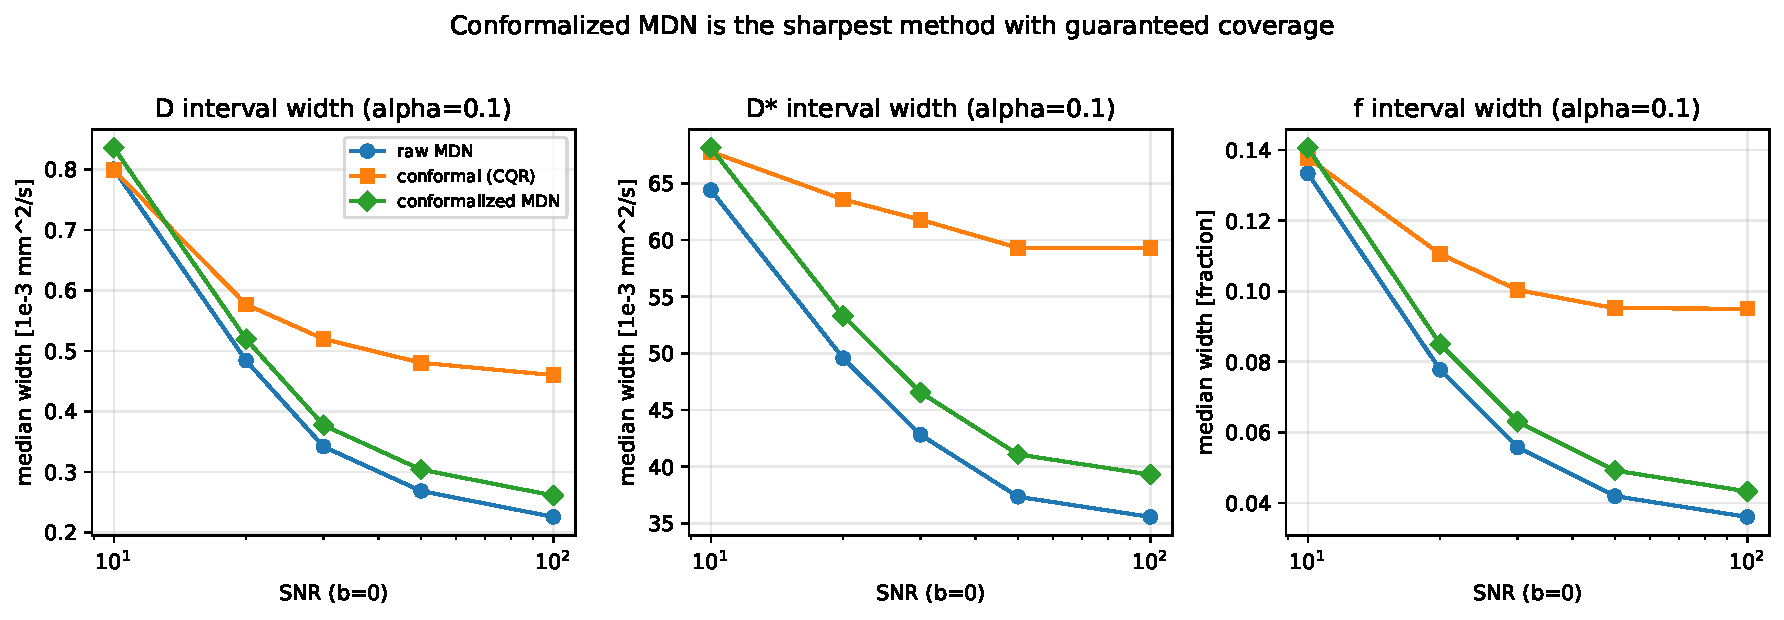
\includegraphics[width=0.78\linewidth]{figures/sharpness_vs_snr.pdf}
\caption{Median interval width vs SNR. Conformalized-MDN is the sharpest method
with a guaranteed coverage level.}
\label{fig:sharpness}
\end{figure}

\begin{figure}[h]
\centering
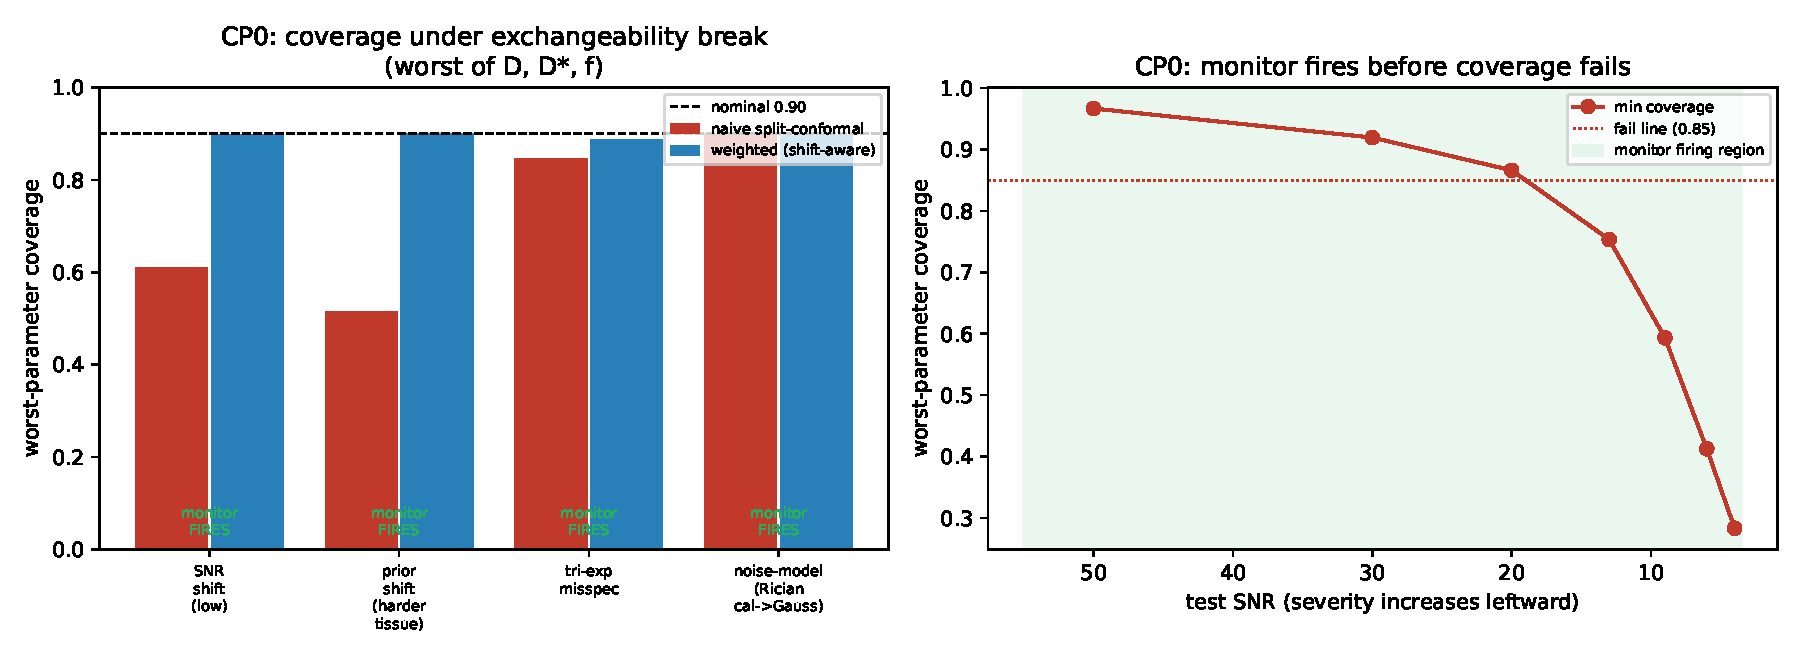
\includegraphics[width=0.92\linewidth]{figures/robustness_shift.pdf}
\caption{(Left) worst-parameter coverage under each exchangeability break, naive
vs.\ weighted, with monitor status. (Right) SNR-severity sweep: the monitor fires
before coverage crosses the failure line.}
\label{fig:shift}
\end{figure}

\begin{figure}[h]
\centering
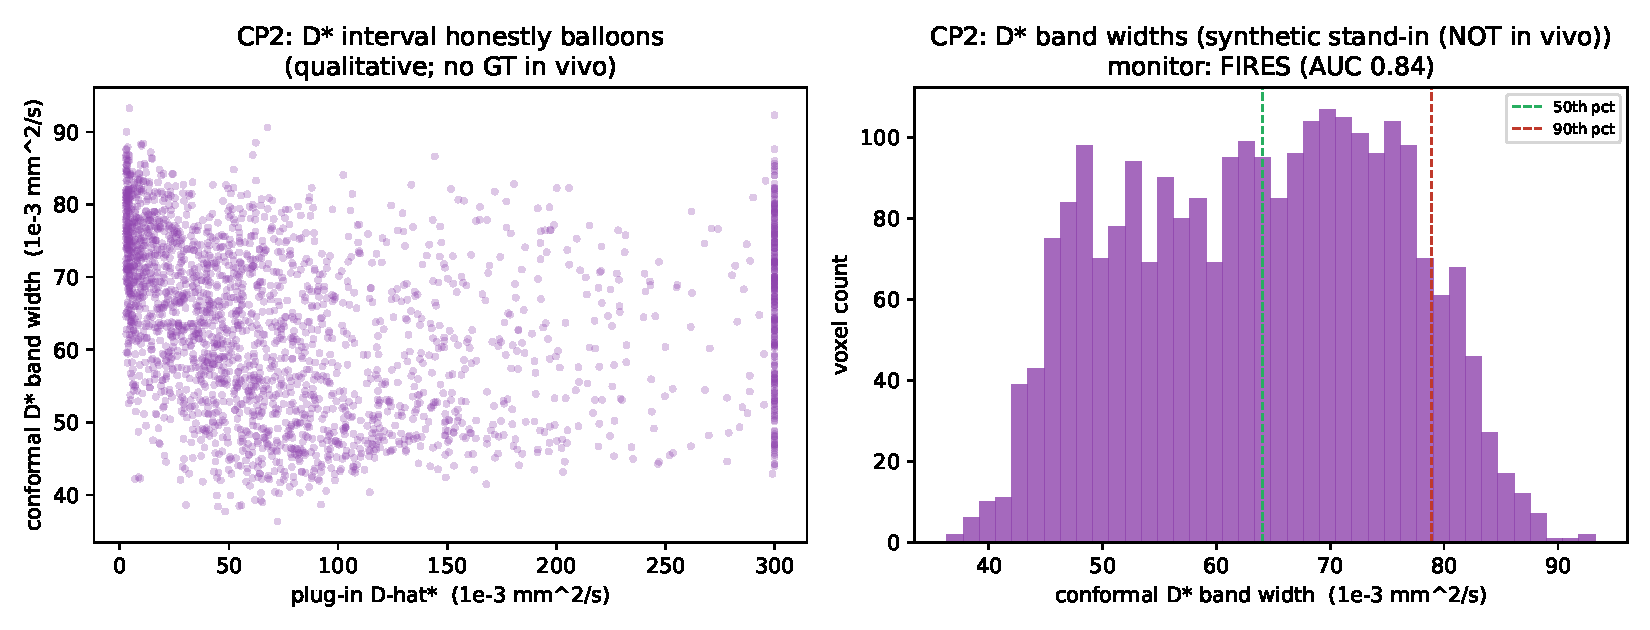
\includegraphics[width=0.92\linewidth]{figures/invivo_demo.pdf}
\caption{In-vivo qualitative demo (synthetic stand-in). (Left) the conformal
$\Dstar$ band balloons with the plug-in $\hat{\Dstar}$. (Right) the heavy-tailed
$\Dstar$ band-width distribution; the deployment monitor fires on the transfer.}
\label{fig:invivo}
\end{figure}

\end{document}
